\documentclass[a4paper]{article}
\usepackage[T2A]{fontenc}
\usepackage[utf8]{inputenc}
\usepackage[ukrainian]{babel}
\usepackage{tikz}
\usepackage{lastpage} 
\usepackage[left=2.5cm, right=1.5cm, top=1.5cm, bottom=2.5cm]{geometry}
\usepackage{fancyhdr}
% \usepackage{graphicx}

\pagestyle{fancy}
\fancyhf{}
\renewcommand{\headrulewidth}{0pt}
\renewcommand{\footrulewidth}{0pt}
% \pagestyle{empty}

\newcommand{\makrosTitle}[2]{
\thispagestyle{empty}
        \centering
        \textbf{Міністерство освіти і науки України}\\
        \textbf{КИЇВСЬКИЙ ПОЛІТЕХНІЧНИЙ УНІВЕРССИТЕТ}\\[2cm]
        \raggedleft
        Кафедра автоматизації та систем неруйнівного контролю\\
        Група ПМ-11
        \vfill
        \centering
        \textbf{ПРОЕКТУВАННЯ СИСТЕМ АВТОМАТИЗАЦІЇ}\\[1cm]
        \textbf{ЗВІТ З ЛАБОРАТОРНОЇ РОБОТИ №#1}\\[1cm]
        \textbf{#2}
        \vfill
        \begin{flushleft}
            Керівник  \qquad\qquad\quad \hfill\qquad (підпис)\hfill 
            д.т.н., проф. Черепанська І. Ю.\\
            \hfill (дата)\\[2cm]
            Виконавець\hfill (підпис)\hfill Погорєлов Б. Ю.\\
            \hfill (дата)
        \end{flushleft}
        \vfill
        \centering
        2025
}

\newcommand{\makrosFrameBig}[2]{
    \thispagestyle{empty} % Вимикає номер сторінки на першій сторінці
    
    \begin{tikzpicture}[remember picture, overlay]
        \begin{scope}[shift={([xshift = 20 mm, yshift = 10 mm]current page.south west)}]
            \draw[line width=2] (0,0) rectangle (180 mm,277 mm);
        \end{scope}
    \end{tikzpicture}
    
    \begin{tikzpicture}[remember picture, overlay]
        \begin{scope}[shift={([xshift = 20 mm, yshift = 10 mm]current page.south west)}, x=1mm, y=1mm]
            \draw[line width=2] (0,0) rectangle (180,40);
            \draw[line width=2]  (7,40) -- (7, 25);
            \draw[line width=2] (17,40) -- (17, 0);
            \draw[line width=2] (40,40) -- (40, 0);
            \draw[line width=2] (55,40) -- (55, 0);
            \draw[line width=2] (65,40) -- (65, 0);
            \draw[line width=2] (135,25) -- (135,0);
            \draw[line width=2] (140,15) -- (140,20);
            \draw[line width=2] (145,15) -- (145,20);
            \draw[line width=2] (150,25) -- (150,15);
            \draw[line width=2] (165,25) -- (165,15);
        
            \draw (0,35) -- (65, 35);
            \draw[line width=2] (0,30) -- (65, 30);
            \draw[line width=2] (0,25) -- (180, 25);
            \draw (0,20) -- (65, 20);
            \draw (0,15) -- (65, 15);
            \draw (0,10) -- (65, 10);
            \draw (0,5) -- (65, 5);
        
            \draw[line width=2] (135,20) -- (180, 20);
            \draw[line width=2] (135,15) -- (180, 15);
            
            \node at (3.5, 27.5) {Зм.};
            \node at (12, 27.5) {Лист};
            \node at (28.5, 27.5) {№ докум.};
            \node at (47.5, 27.5) {Підпис};
            \node at (60, 27.5) {Дата};
            
            \node at (7, 22.5) {Розроб.};
            \node at (6.5, 17.5) {Перев.};
            \node at (8.5, 7.5) {Н. Контр.};
            \node[align=left] at (5, 2.5) {Затв.};
            
            \node at (142.5, 22.5) {Літ.};
            \node at (157.5, 22.5) {Аркуш};
            \node at (172, 22.5) {Аркушів};
        
            \node[align=left, font=\itshape, anchor=south west, scale=0.9] at (16, 20) {Погорєлов Б.Ю.};
            \node[align=left, font=\itshape, anchor=south west, scale=0.8] at (16, 15) {Черепанська І.Ю.};
            \node[align=left, font=\itshape, anchor=south west, scale=0.8] at (16, 0) {Черепанська І.Ю.};
        
            \node[anchor=center, font=\itshape, scale=1.5] at (122, 32) {#1};
            \node[align=center, font=\itshape, anchor=center] at (100, 12) {#2};
            \node[align=left, font=\itshape, anchor=south west, scale=0.9] at (135, 5) {КПІ ім. І. Сікорського, ПБФ};
            \node[anchor=center, font=\itshape] at (158, 17) {2};
            \node[anchor=center, font=\itshape] at (172, 17) {\pageref{LastPage}};    
        \end{scope} 
    \end{tikzpicture}
}

\newcommand{\makrosFrameSmall}[1]{
    % \thispagestyle{empty} % Вимикає номер сторінки на першій сторінці
    
    \begin{tikzpicture}[remember picture, overlay]
        \begin{scope}[shift={([xshift = 20 mm, yshift = 10 mm]current page.south west)}]
            \draw[line width=2] (0,0) rectangle (180 mm,277 mm);
        \end{scope}
    \end{tikzpicture}
    
    \begin{tikzpicture}[remember picture, overlay]
        \begin{scope}[shift={([xshift = 20 mm, yshift = 10 mm]current page.south west)}, x=1mm, y=1mm]
            \draw[line width=2] (0,0) rectangle (180,15);
            \draw[line width=2] (7,0) -- (7, 15);
            \draw[line width=2] (17,0) rectangle (43,15);
            \draw[line width=2] (55,0) rectangle (64,15);
            \draw[line width=2] (170,0) -- (170, 15);

            \draw[line width=2] (0,5) -- (64, 5);
            \draw               (0,10) -- (64, 10);
            \draw[line width=2] (170,8) -- (180, 8);

            \node[anchor=center, scale=0.8] at (3.5, 2.5) {Змн.};
            \node[anchor=center, scale=0.9] at (12, 2.5) {Арк.};
            \node[anchor=center] at (30, 2.5) {№~докум.};
            \node[anchor=center, scale=0.9] at (49, 2.5) {Підпис};
            \node[anchor=center, scale=0.9] at (59, 2.5) {Дата};
            \node[anchor=center, font=\itshape, scale=1.5] at (115, 7.5) 
                {#1};
            \node[anchor=center] at (175, 12) {Арк.};
            \node[anchor=center] at (175, 4) {\thepage};
            
        \end{scope}
    \end{tikzpicture}
}

% \makrosLab{1}{Шифр}{Назва}
\newcommand{\makrosLab}[3]{ 
    \fancyfoot[C]{\makrosFrameSmall{#2}}
    \makrosTitle{#1}{#3}
    \newpage
    \makrosFrameBig{#2}{#3}
    \raggedright
}


\begin{document}
    \makrosLab{1}{л}{
        Використання сучасних програмних \\
        засобів для автоматизованого \\
        проектування систем автоматизації
    }

    \section*{Тема роботи}
    Використання сучасних програмних засобів для автоматизованого проектування систем автоматизації.

    \section*{Мета роботи} 
    Метою моєї роботи було ознайомлення з деякими відомими сучасними САПР і набуття практичних навичок 
    у їх використанні для вирішення типових інженерних завдань, зокрема для розробки електричних 
    принципових схем за допомогою програмного продукту Splan 7.0.
 
    \section*{Варіант 9}

    \section*{Хід роботи}
    Першим етапом роботи стало ознайомлення з теоретичними відомостями щодо програмних засобів для 
    автоматизованого проектування (САПР). Я вивчив основні функції програм, таких як Splan 7.0, які 
    дозволяють ефективно розробляти електричні принципові схеми. Важливим аспектом є можливість 
    створювати схеми, що відповідають вимогам державних стандартів.

    Далі я приступив до використання програми Splan 7.0 для створення електричної принципової схеми 
    згідно з моїм індивідуальним завданням. Я вибрав відповідний тип схеми, визначив елементи та їх 
    взаємозв'язки, після чого приступив до нанесення елементів на схему. Кожен елемент я ретельно 
    позначав відповідно до вимог стандартів ЄСКД, що включають точні позначення компонентів електричних 
    схем, що є важливим для правильного розуміння та подальшого використання схеми.

    Після розробки схеми я створив нові елементи бібліотеки, що дозволило мені розширити можливості 
    програми та врахувати специфіку завдання. Створення бібліотеки елементів є важливим етапом, 
    оскільки дозволяє заощадити час при подальшій роботі та дає змогу швидко додавати нові компоненти 
    до проекту.

    \begin{figure}[h]
        \centering
        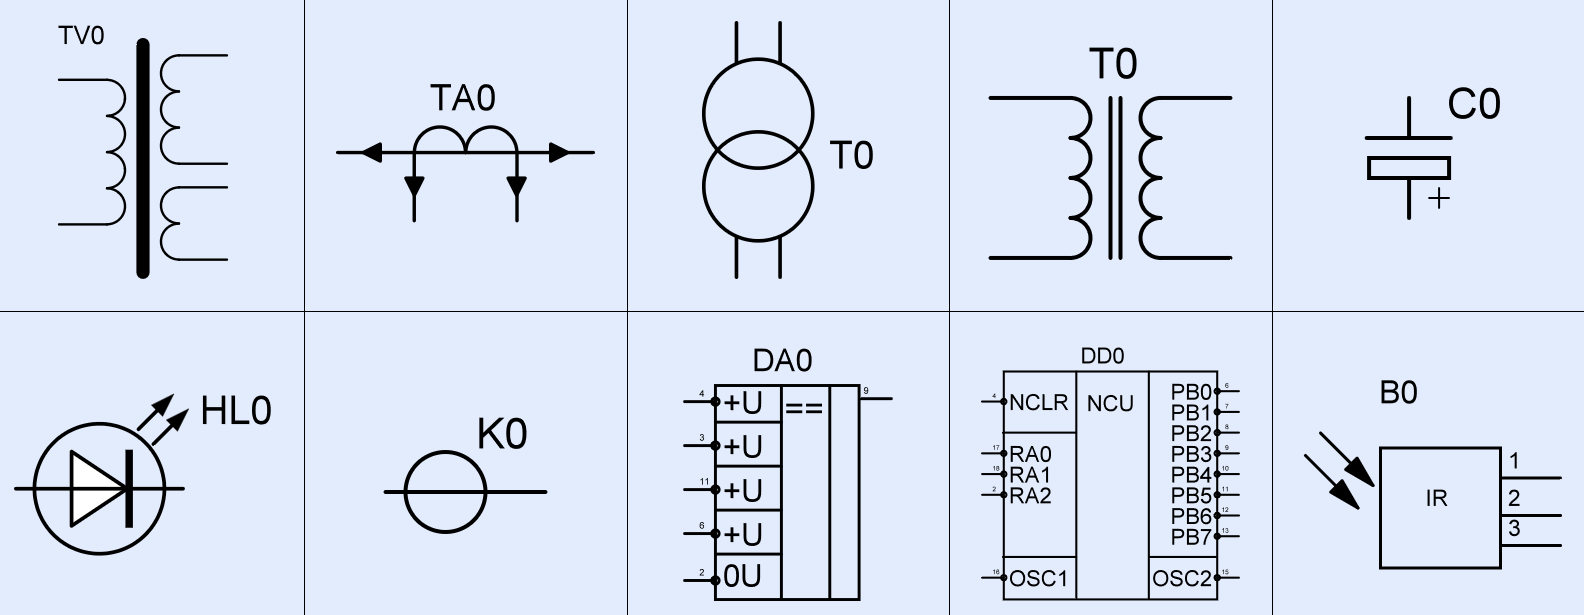
\includegraphics[width=1\textwidth]{imgs/LW1.1.png}
        \caption*{Рис 1.1: Елементи створеної бібліотеки}
    \end{figure} 

    \newpage 
 
    \begin{figure}[h]
        \centering
        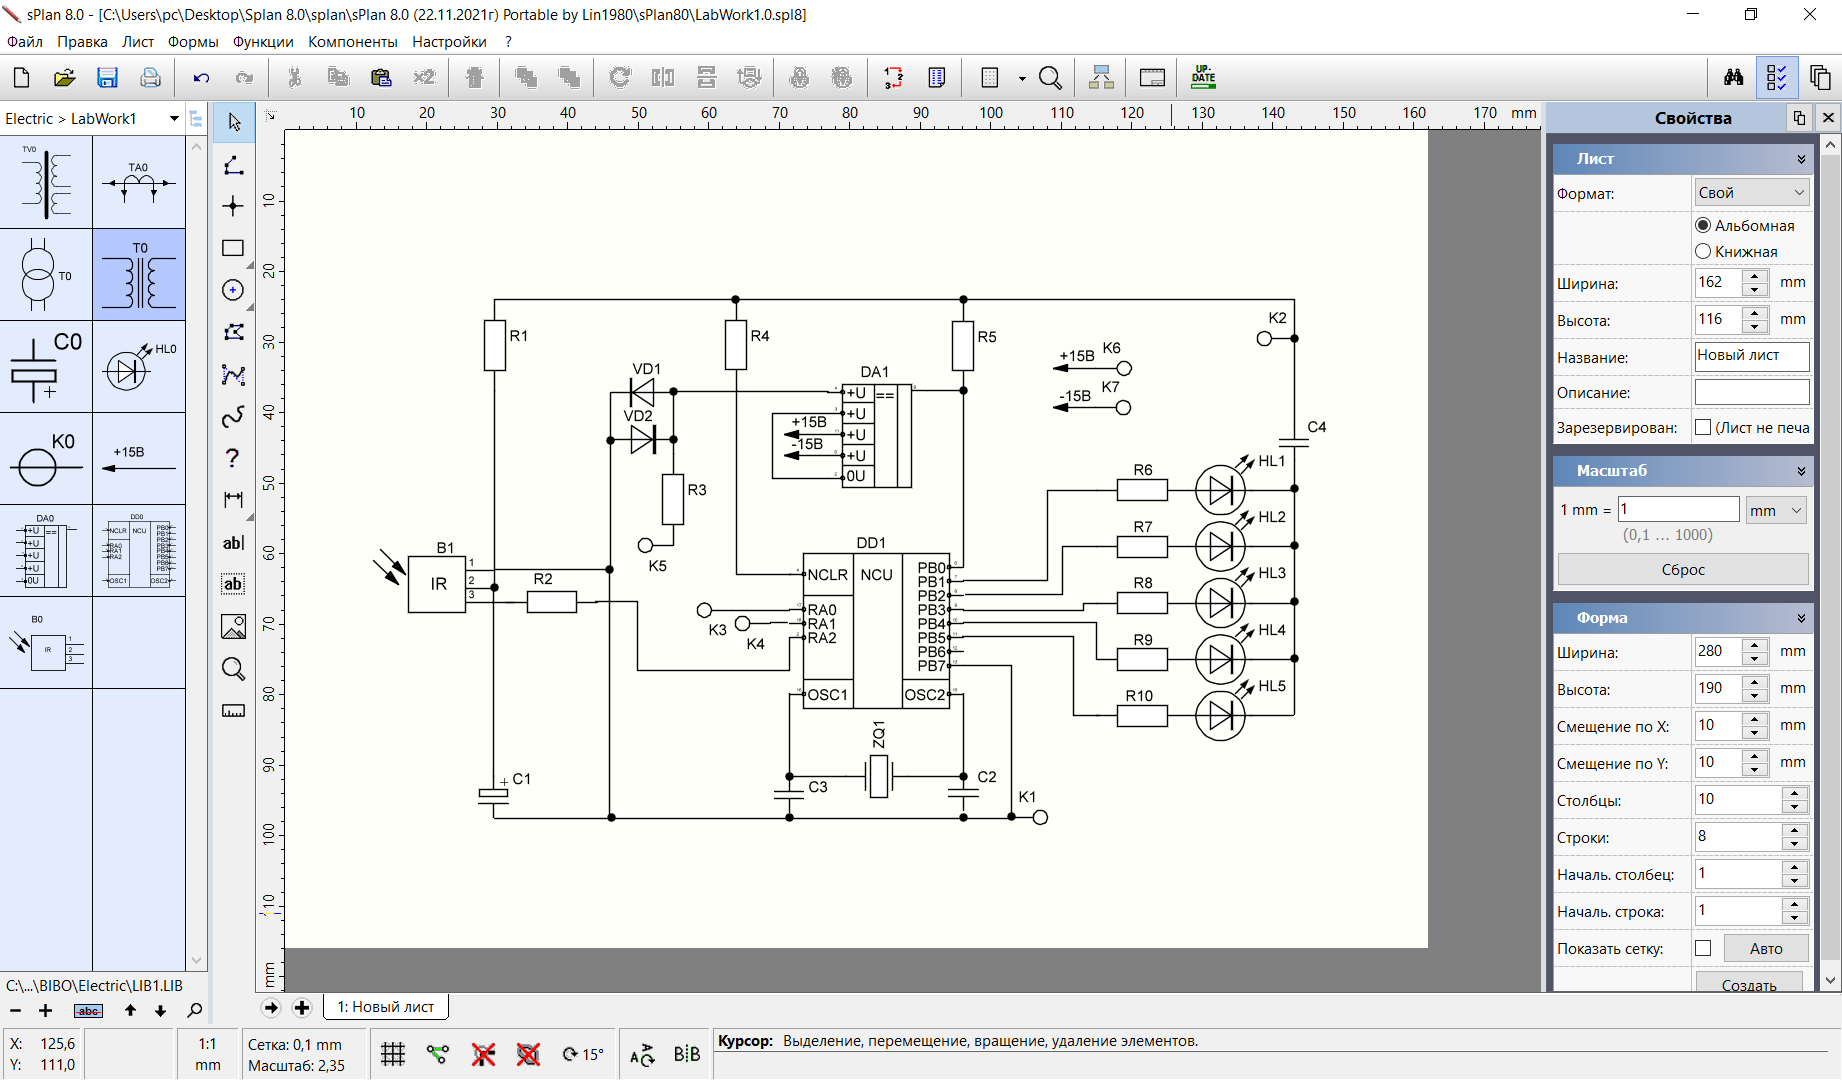
\includegraphics[width=1\textwidth]{imgs/LW1.3.png}
        \caption*{Рис 1.2: Електрична схема}
    \end{figure} 

    \section*{Висновок}
    В результаті виконаної роботи я ознайомився з основними функціями програмного забезпечення 
    для автоматизованого проектування, зокрема Splan 7.0. Я набув практичних навичок у створенні 
    електричних принципових схем та освоїв процес позначення елементів згідно з державними стандартами. 
    Також я створив новий елемент бібліотеки, що допомогло покращити ефективність роботи в програмі. 
    В цілому, робота дозволила мені краще зрозуміти можливості сучасних САПР та їх використання для 
    розв'язання типових інженерних завдань.

    \section*{1.3. Контрольні питання}
    \begin{enumerate}
        \item \textbf{Що забезпечує САПР?} \\
        САПР (система автоматизованого проектування) забезпечує автоматизацію процесів проектування, 
        що включає створення, редагування та аналіз різних видів технічних схем, розрахунків і моделей. 
        Вона значно зменшує час, необхідний для проектних робіт, підвищує точність та якість проектування, 
        а також дозволяє створювати проекти, які відповідають стандартам.

        \item \textbf{Що означає САD?} \\
        САD (Computer-Aided Design) — це система комп'ютерного проектування, яка використовується для 
        створення, зміни, аналізу та оптимізації проектів. САПР є частиною цієї системи і охоплює програмні 
        засоби, які допомагають проектувати різні технічні об'єкти, зокрема електричні схеми.

        \item \textbf{Чому електричні схеми складають за вимогами ЄСКД?} \\
        ЄСКД (Єдина система конструкторської документації) визначає стандарти та вимоги до оформлення 
        технічної документації. Електричні схеми складають за цими вимогами для того, щоб забезпечити 
        уніфікацію позначень елементів, зрозумілість для інших спеціалістів, а також відповідність всім 
        нормативам та стандартам в галузі.

        \item \textbf{Що таке ЄСКД?} \\
        ЄСКД (Єдина система конструкторської документації) — це система, що включає стандарти і норми 
        для розробки та оформлення проектної документації. Вона визначає вимоги до зовнішнього вигляду 
        документів, позначення елементів, а також правила виготовлення креслень та схем, що забезпечують 
        правильне розуміння та використання документів.
    \end{enumerate}

\end{document}